\documentclass[11p, titlepage, oneside, a4paper]{article}
% Packages
\usepackage{amsmath}
\usepackage{graphicx}
\usepackage{hyperref}
\usepackage[english,swedish]{babel}
\usepackage[
    backend=biber,
    style=authoryear-ibid,
    sorting=ynt
]{biblatex}
\usepackage[utf8]{inputenc}
\usepackage[T1]{fontenc}
%Källor
\addbibresource{mall.bib}
\graphicspath{ {./images/} }

% Ändra de rader som behöver ändras
\def\inst{Teknikprogrammet}
\def\typeofdoc{Laborationsrapport}
\def\course{Fysik 1 150p}
\def\pretitle{Laboration 2}
\def\title{Kraft: Friktionskraft och fjäderkraft}
\def\name{Axel Jakobsson}
\def\username{axel.jakobsson}
\def\email{\username{}@ga.ntig.se}
\def\graders{Magnus Silverdal}

\begin{document}

    \begin{titlepage}
        \thispagestyle{empty}
        \begin{large}
            \begin{tabular}{@{}p{\textwidth}@{}}
                \textbf{NTI gymnasiet \hfill \today} \\
                \textbf{\inst} \\
                \textbf{\typeofdoc} \\
            \end{tabular}
        \end{large}
        \vspace{10mm}
        \begin{center}
            \LARGE{\pretitle} \\
            \huge{\textbf{\course}}\\
            \vspace{10mm}
            \LARGE{\title} \\
            \vspace{15mm}
            \begin{large}
                \begin{tabular}{ll}
                    \textbf{Namn} & \name \\
                    \textbf{E-mail} & \texttt{\email} \\
                \end{tabular}
            \end{large}
            \vfill
            
\includegraphics[width=0.5\textwidth]{images/NTI Gymnasiet_Symbol_print_svart.png}
            \vfill
            \large{\textbf{Handledare}}\\
            \mbox{\large{\graders}}
        \end{center}
    \end{titlepage}

    \begin{otherlanguage}{english}
        \begin{abstract}
             In the first experiment a block slid down an inclining plane at a constant speed. This allowed us to get a connection between the Frictions force to the relation of the neutral force. The experiment was repeated 4 more times with another weight on it each time (50g). The results were noted down and turned into a diagram.
            In the second experiment a spring was hung on a hook and the length was noted down. Then the experiment was repeated 4 times whilst adding a weight (50g) each time and noting down the new length of the feather. With this data a diagram was created of the relation between the springs force and the length.
        \end{abstract}
    \end{otherlanguage}
    % Om arbetet är långt har det en innehållsförteckning, annars kan den utelämnas
    \pagenumbering{roman}
    \tableofcontents

    % och lägger in en sidbrytning
    \newpage

    \pagenumbering{arabic}

    % i Sverige har vi normalt inget indrag vid nytt stycke
    \setlength{\parindent}{0pt}
    % men däremot lite mellanrum
    \setlength{\parskip}{10pt}

    \section{Syfte och frågeställning}
    Syftet med första laborationstestet var att räkna ut friktionskraften i förhållande till neutralkraften. Syftet med andra laborationsexperimentet var att räkna ut sambandet mellan fjäderkraften och dens längd.

    \section{Bakgrund och teori}
    För att få resultaten för det första laborationsexperimentet, friktionsexperimentet så mättes en kloss som låg på en träplanka. Träplankan lyftes på en sida tills att klossen började röra sig i konstant hastighet. Sedan upprepades experimentet 4 gånger till, med en extra vikt (50g) för varje nytt försök.
    I det andra experimentet så mättes en fjäders längd medans den hängde i en krok. Experimentet upprepades 4 gånger till och en vikt (50g) lades till på fjädern.

    \section{Metod och materiel}
    \begin{enumerate}
        Första experimentet:
        \item Kloss
        \item En träplanka
        \item Linjal
        \item Vikter
        Andra experimentet:
        \item Fjäder
        \item Vikter
        \item Linjal
    \end{enumerate}




    \newpage
    \section{Analys och beräkning}
    Från resultaten av experimenten så har ett diagram skapats för båda två. Diagrammet för friktionskraften är här \ref{fig:friktion} och diagrammet för fjäderkraften finns här \ref{fig:fjader}. I friktionsdiagrammet så ser vi sambandet mellan Friktionskraften och Normalkraften. I Fjäderkraftens diagram så visas sambandet mellan fjäderkraften och längden i cm.

    \begin{figure}
        \centering
        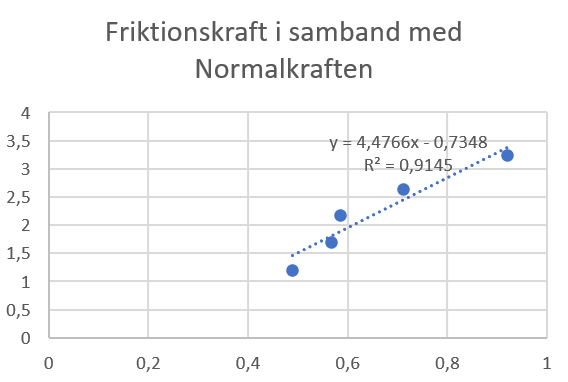
\includegraphics[scale=0.1]{images/friktionskraft}
        \caption{}
        \label{fig:friktion}
    \end{figure}
    \begin{figure}
        \centering
        \includegraphics[scale= 0.1]{images/fjäderkraft}
        \caption{}
        \label{fig:fjäder}
    \end{figure}




    Datat importeras i Excel och Friktionskraften beräknas med hjälp av formeln: tyngdkraften*sin(vinkeln). Normalkraften räknades ut med ekvationen: Tyngdkraften*cos(vinkeln). Fjäderkraften räknades ut med ekvationen: massa*9,82.

    \section{Slutsats och resultat}
    Resultatet av beräkningarna illustreras i graferna 2 och 3
    \section{Diskussion}
    Resultatet är perfekt...


    \printbibliography

\end{document}

